\section{Problem Formulation}
\label{sec:problem}

\subsection{Dec-POMDP Definition}
\label{sec:decpomdp}
We formulate cooperative multi-intersection signal control as a Decentralized
Partially Observable Markov Decision Process
(Dec-POMDP)~\cite{oliehoek2016_decpomdp}
\begin{equation}
  \langle \mathcal{N}, \mathcal{S}, \{\mathcal{A}_i\}, \{\mathcal{O}_i\},
  \mathcal{P}, \mathcal{R}, \gamma \rangle,
  \qquad
  \mathcal{A} \equiv \prod_{i=1}^{N} \mathcal{A}_i,
  \label{eq:joint_action}
\end{equation}
with standard semantics: one homogeneous agent per signalized intersection, a global
state $\mathcal{S}$ that encodes the microscopic configuration of every vehicle and
signal, a transition kernel $\mathcal{P}$ that also enforces all safety-critical signal
timing, a per-agent scalar reward $r_{i,t}$, and $\gamma = 0.99$. The two components
central to this work are the binary per-agent action space $\mathcal{A}_i = \{0, 1\}$
(Section~\ref{sec:action_space}) and the local observation space $\mathcal{O}_i$, the
$26$-dimensional camera-computable proxy of Section~\ref{sec:obs_space}. Agents act
every $\Delta t = 5$~s over $1080$ decision steps ($5400$~s) per episode. The state
$\mathcal{S}$ is available only in simulation; reconciling it with what a deployed
controller can actually sense motivates the projection developed next.

\subsection{The Observation Projection}
\label{sec:projection}
A critical challenge in deploying RL-based signal control is the discrepancy between
the privileged training state and the limited local observations available on
hardware. The global state $\mathbf{s}_t \in \mathcal{S}$ exposes quantities---exact
per-vehicle accumulated waiting times, network-wide arrival counts---that no roadside
camera can recover at inference time. We treat this discrepancy as a fundamental
design constraint rather than a post-hoc adaptation, and delineate the privileged
state from each local observation $\mathbf{o}_{i,t} \in \mathcal{O}_i$ through an
explicit camera-computable projection $\phi_i$,
\begin{equation}
  \mathbf{o}_{i,t} = \phi_i(\mathbf{s}_t) + \varepsilon_{i,t},
  \label{eq:projection}
\end{equation}
where $\phi_i$ retains only state components an overhead camera can estimate and
$\varepsilon_{i,t}$ encapsulates the sensing noise of the vision pipeline. Training
uses the noiseless projection ($\varepsilon_{i,t} = \mathbf{0}$); the perturbed regime
is reserved for the robustness evaluation and physical deployment.

This projection imposes a single design rule in two places. The execution policy
factors entirely through it,
\begin{equation}
  a_{i,t} \sim \pi_\theta\!\left(\cdot \mid \mathbf{o}_{i,t}\right),
  \label{eq:policy}
\end{equation}
so the actor consumes exactly the inputs available on-camera. The \emph{training
objective} obeys the same restriction: every reward component admits a
$\phi$-computable estimator, eliminating privileged simulator reads from the entire
training loop. This requirement distinguishes the present formulation from prior
vision-based RL-TSC methods, which restrict the observation yet still optimize against
privileged lane-delays or throughput drawn from the
simulator~\cite{dai2022_worldmodels, azfar2025_cosim}.

\subsection{Observation Space}
\label{sec:obs_space}
The observation space $\mathcal{O}_i$ is a $26$-dimensional vector that aggregates
traffic metrics at the \emph{approach} level. We adopt approach-level rather than
lane-level features because lane abstractions break down under motorcycle-dominant
traffic, where vehicles filter between and swarm across nominal lane boundaries; the
approach grouping instead matches the macroscopic field of view of one camera Region
of Interest (ROI). For each of the $4$ incoming approaches we extract $5$ features
normalized to $[0, 1]$---effective halted-queue length, spatial occupancy, average
vehicle speed, motorcycle share, and heavy-vehicle share---yielding $20$ dimensions.
The remaining $6$ dimensions encode the controller state: a $4$-dimensional phase
one-hot vector, a normalized green timer, and a scalar \emph{phase-imbalance}
feature $\mathrm{pressure\_norm}$ that summarizes the local demand imbalance
between the two phase groups at the same junction---an intra-junction
quantity, not the upstream--downstream network pressure of classical
max-pressure control~\cite{varaiya2013_maxpressure},
\begin{equation}
  \mathrm{pressure\_norm}
  = \max\!\left(0,\; \min\!\left(1,\; \tfrac{1}{2}\left(1 + \bar{q}_A - \bar{q}_B\right)\right)\right),
  \label{eq:pressure_norm}
\end{equation}
where
\begin{equation}
  \bar{q}_G = \frac{1}{|G|} \sum_{l \in G} q_l
  \label{eq:group_queue}
\end{equation}
is the mean normalized queue over phase group $G \in \{A, B\}$. The group \emph{mean}
renders the feature invariant to asymmetric approach counts, so that
$\mathrm{pressure\_norm} = \tfrac{1}{2}$ denotes a balanced network and deviations
identify the congested group. Each approach feature maps to a documented camera
estimator---queue from near-stationary bounding boxes ($v\approx 0$), occupancy from the summed box footprint, speed from per-track displacement under ByteTrack~\cite{zhang2022_bytetrack}, and class shares
from YOLOv11 detections~\cite{khanam2024_yolov11, ultralytics_yolo11}---against
simulator counterparts read from SUMO's sublane model~\cite{lopez2018_sumo}, as
summarized in Table~\ref{tab:obs_space}.
\begin{table}[htbp]
  \centering
  \caption{26-Dimensional Local Proxy Observation Space ($\mathcal{O}_i$). Each
  approach feature occupies index $5k{+}j$ for approach $k\in\{0,1,2,3\}$ and
  feature $j$; the four approaches fill indices $0$--$19$.}
  \label{tab:obs_space}
  \vspace{-4mm}
  \resizebox{\columnwidth}{!}{%
  \begin{tabular}{clllc}
    \toprule
    \textbf{Index} & \textbf{Feature} & \textbf{Simulator Source} & \textbf{Camera Estimator} & \textbf{Proxy?}\\
    \midrule
    $5k{+}0$ & \texttt{effective\_queue} & $\Sigma$ halted len./lane len. & Near-stationary box len. & Yes\\
    $5k{+}1$ & \texttt{occupancy\_norm}  & Lane occupancy (1D)            & Summed box-length ratio  & Yes\\
    $5k{+}2$ & \texttt{avg\_speed\_norm} & Mean tracked speed    & Track displacement    & Yes\\
    $5k{+}3$ & \texttt{motorbike\_share} & Count by vType        & YOLO \emph{motorcycle}& Yes\\
    $5k{+}4$ & \texttt{heavy\_veh\_share}& Count by vType        & YOLO \emph{truck, bus}& Yes\\
    \midrule
    20--23 & \texttt{phase\_one\_hot}  & Controller state      & Internal variable     & --\\
    24     & \texttt{green\_timer}     & Controller state      & Internal variable     & --\\
    25     & \texttt{pressure\_norm}   & Aggregated queues     & Aggregated proxy      & --\\
    \bottomrule
  \end{tabular}}
\end{table}
The end-to-end proxy construction is visualized later in Figure~\ref{fig:architecture} as
part of the overall system architecture.

\subsection{Action Space and Signal Constraints}
\label{sec:action_space}
The per-agent action space is binary, $\mathcal{A}_i = \{0,1\}$, selecting which of
two non-conflicting phase groups---Group~A or Group~B, whose approach membership is
fixed by the intersection phase plan---receives the right-of-way; this abstraction
matches the legacy two-phase hardware prevalent in developing-city corridors. The
agent decides only \emph{which} group is served, not \emph{when} transitions occur:
$\mathcal{P}$ enforces a mandatory $3$~s yellow clearance on every switch and a
$15$~s minimum green, overriding (by holding the current phase) any switch requested
before the minimum green has elapsed. The sampled action and its log-probability
enter the rollout buffer while the switch penalty is keyed to the \emph{realized}
switch indicator, so credit assignment under the override remains consistent and no
spurious penalty is incurred. The $60$~s maximum green is \emph{not} a forced switch;
it caps the accumulated green timer and sets the normalization scale of the
\texttt{green\_timer\_norm} feature (Section~\ref{sec:obs_space}), leaving
cross-movement starvation to the reward shaping (Section~\ref{sec:reward}) and
cleanly separating learned phase selection from operational safety.
Figure~\ref{fig:signal_fsm} summarizes this two-phase logic and
the environment-enforced timing.
\begin{figure}[H]
  \centering
  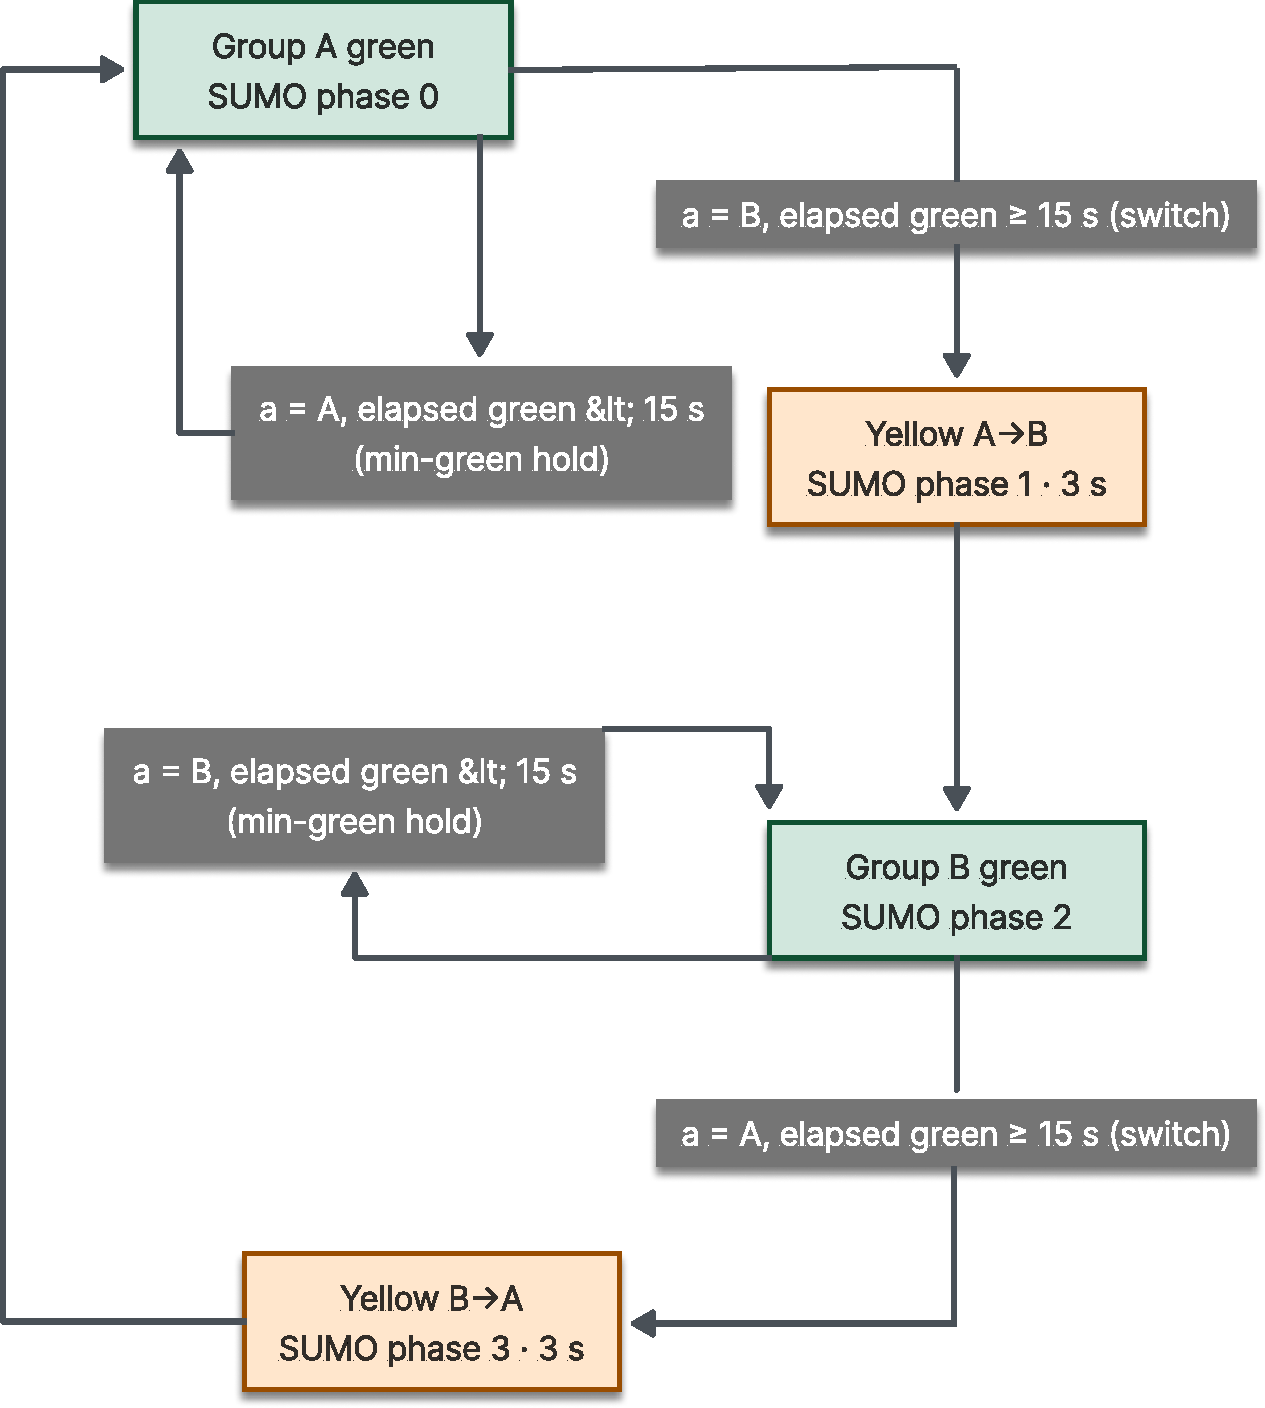
\includegraphics[width=\columnwidth]{assets/figures/fig2.pdf}
   \caption{Two-phase control and environment-enforced timing. At each $5$~s decision
  the binary action selects which non-conflicting group is served. On a switch the
  environment runs a $3$~s yellow clearance and then the new green for the remaining
  $2$~s of the step; the green timer resets to ${\approx}2$~s and accumulates $+5$~s
  per extend, capped at $60$~s. The $15$~s minimum green is a hard constraint, whereas
  the $60$~s maximum only caps the \texttt{green\_timer\_norm} feature and is not a
  forced switch.}
  \label{fig:signal_fsm}
  \vspace{-4mm}
\end{figure}
% NOTE: the Sensing-Noise Model overview (formerly Sec. III-F, \label{sec:noise_model})
% was merged into Sec. VI (Robustness to Sensing Noise) where it is used.